\documentclass[aspectratio=169]{beamer}
\usepackage[T1]{fontenc}
\usepackage[utf8]{inputenc}
\usepackage{lmodern}
\usepackage{microtype}
\usepackage{xcolor}
\usepackage{tikz}
\usetikzlibrary{positioning, arrows.meta, fit, backgrounds, calc}
\usepackage{fontawesome5}

\definecolor{wurgreen}{HTML}{34B233}
\definecolor{darkgreen}{HTML}{1F6B1E}
\definecolor{darknavy}{HTML}{1A1A2E}
\definecolor{midgray}{HTML}{6B7280}
\definecolor{lightgray}{HTML}{F3F4F6}
\definecolor{lightgreen}{HTML}{E8F7E8}
\definecolor{bodytext}{HTML}{1F2937}
\definecolor{warnred}{HTML}{FEE2E2}
\definecolor{warnborder}{HTML}{EF4444}
\definecolor{attnblue}{HTML}{DBEAFE}
\definecolor{attnborder}{HTML}{3B82F6}

\usetheme{default}
\usecolortheme{default}
\usefonttheme{professionalfonts}
\setbeamertemplate{navigation symbols}{}
\setbeamertemplate{itemize items}{\textcolor{wurgreen}{\textbullet}}
\setbeamertemplate{itemize subitem}{\textcolor{midgray}{--}}
\setbeamercolor{frametitle}{fg=white, bg=darknavy}
\setbeamerfont{frametitle}{size=\large, series=\bfseries}
\setbeamertemplate{frametitle}{%
  \begin{beamercolorbox}[wd=\paperwidth, ht=1.1cm, dp=0.2cm, leftskip=0.6cm]{frametitle}
    \usebeamerfont{frametitle}\insertframetitle
  \end{beamercolorbox}}
\setbeamercolor{background canvas}{bg=white}
\setbeamercolor{normal text}{fg=bodytext}
\setbeamertemplate{footline}{%
  \begin{beamercolorbox}[wd=\paperwidth, ht=0.4cm, dp=0.15cm]{footline}
    \hspace{0.5cm}\textcolor{midgray}{\tiny Bags, Vectors \& Transformers · Wageningen University \& Research}%
    \hfill\textcolor{midgray}{\tiny \insertframenumber}\hspace{0.4cm}
  \end{beamercolorbox}}

\begin{document}

% ── TITLE ──────────────────────────────────────────────────────────────────
{
\setbeamertemplate{footline}{}
\begin{frame}[plain]
  \begin{tikzpicture}[remember picture, overlay]
    \fill[darknavy] (current page.south west) rectangle (current page.north east);
    \fill[wurgreen] (current page.south west) rectangle
      ([xshift=0.45cm]current page.north west);
    \node[anchor=west, text=white, font=\huge\bfseries, text width=13cm]
      at ([xshift=1.1cm, yshift=1.2cm]current page.west)
      {Bags, Vectors \& Transformers};
    \node[anchor=west, text=wurgreen, font=\large, text width=12cm]
      at ([xshift=1.1cm, yshift=0.05cm]current page.west)
      {Contextual Embeddings \& Transformers · Day 3};
    \node[anchor=west, text=midgray, font=\small, text width=12cm]
      at ([xshift=1.1cm, yshift=-1.5cm]current page.west)
      {Denise J. Roth, PhD Candidate\\
       Strategic Communication Group · Wageningen University \& Research};
  \end{tikzpicture}
\end{frame}
}

% ── SLIDE 1: recap ────────────────────────────────────────────────────────
\begin{frame}{Where We Have Been}
\vspace{0.2cm}
{\small Two days, one journey --- from counting words to representing meaning:}

\medskip
\begin{columns}[T]
  \column{0.31\textwidth}
  \vspace{0pt}
  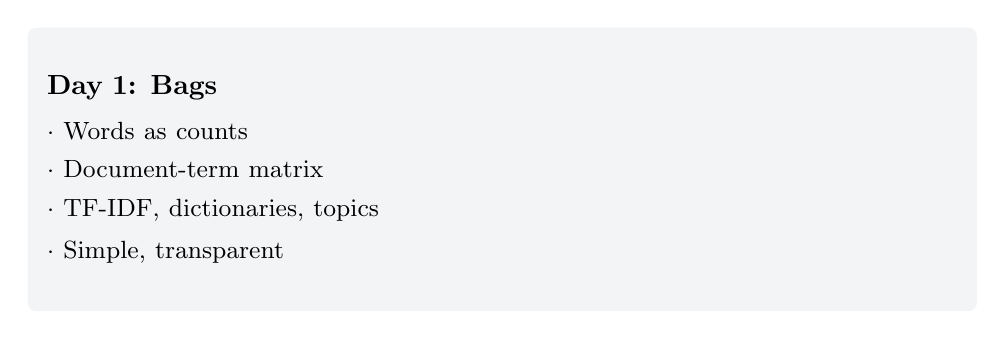
\begin{tikzpicture}
    \node[fill=lightgray, rounded corners=3pt,
          inner xsep=7pt, inner ysep=8pt, text width=\columnwidth-16pt, minimum height=3.6cm]{%
      \textbf{Day 1: Bags}\\[5pt]
      {\small
      $\cdot$ Words as counts\\[3pt]
      $\cdot$ Document-term matrix\\[3pt]
      $\cdot$ TF-IDF, dictionaries, topics\\[3pt]
      $\cdot$ Simple, transparent}};
  \end{tikzpicture}

  \column{0.31\textwidth}
  \vspace{0pt}
  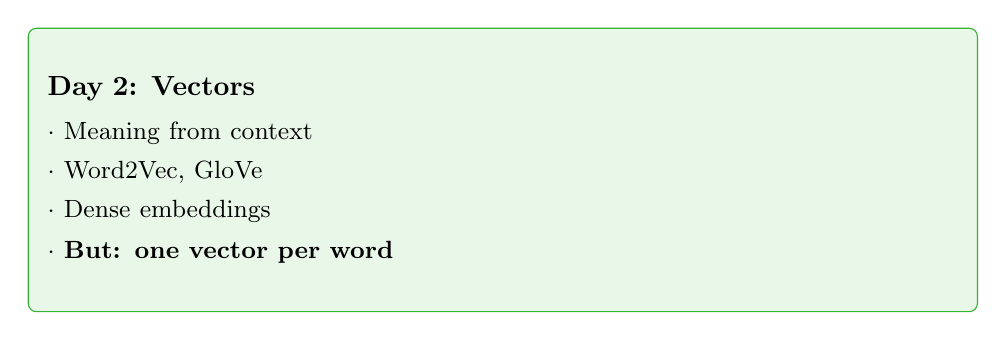
\begin{tikzpicture}
    \node[fill=lightgreen, draw=wurgreen, rounded corners=3pt,
          inner xsep=7pt, inner ysep=8pt, text width=\columnwidth-16pt, minimum height=3.6cm]{%
      \textbf{Day 2: Vectors}\\[5pt]
      {\small
      $\cdot$ Meaning from context\\[3pt]
      $\cdot$ Word2Vec, GloVe\\[3pt]
      $\cdot$ Dense embeddings\\[3pt]
      $\cdot$ \textbf{But: one vector per word}}};
  \end{tikzpicture}

  \column{0.31\textwidth}
  \vspace{0pt}
  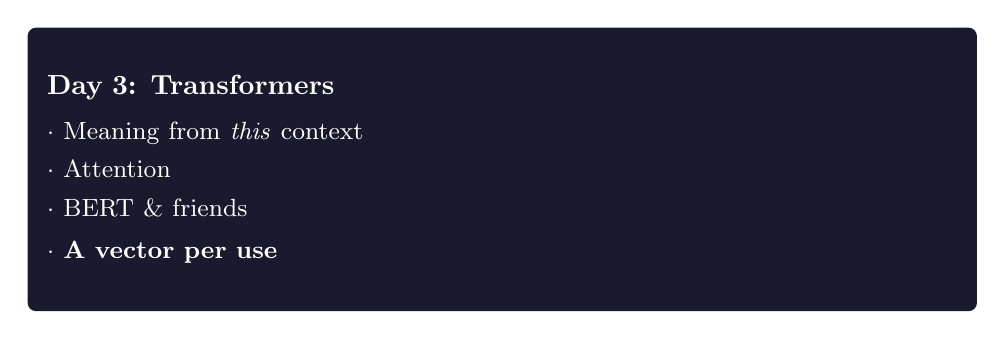
\begin{tikzpicture}
    \node[fill=darknavy, rounded corners=3pt,
          inner xsep=7pt, inner ysep=8pt, text width=\columnwidth-16pt, minimum height=3.6cm]{%
      \textcolor{white}{\textbf{Day 3: Transformers}}\\[5pt]
      {\small\color{white}
      $\cdot$ Meaning from \emph{this} context\\[3pt]
      $\cdot$ Attention\\[3pt]
      $\cdot$ BERT \& friends\\[3pt]
      $\cdot$ \textbf{A vector per use}}};
  \end{tikzpicture}
\end{columns}

\medskip
{\small\textcolor{midgray}{\textit{Today we close the loop: the context problem that static
embeddings could not solve.}}}
\end{frame}

% ── SLIDE 2: the recap of the problem ─────────────────────────────────────
\begin{frame}{The Problem, One More Time}
\vspace{0.2cm}
{\small Static embeddings give each word \textbf{one fixed vector}. But words change meaning
with context --- and a single vector cannot be in two places at once.}

\medskip
\begin{center}
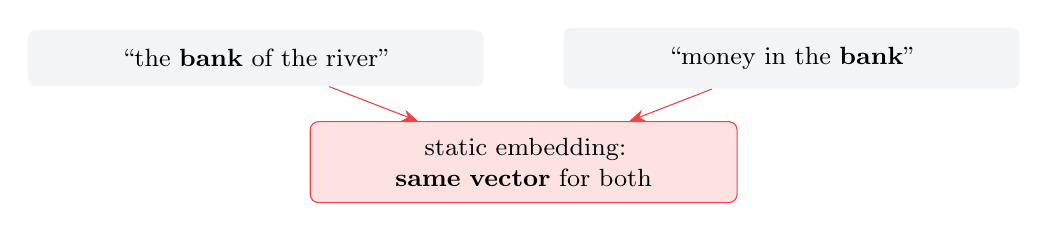
\begin{tikzpicture}[font=\small]
  \node[fill=lightgray, rounded corners=3pt, inner sep=7pt, text width=5.3cm, align=center] (s1)
    {``the \textbf{bank} of the river''};
  \node[fill=lightgray, rounded corners=3pt, inner sep=7pt, text width=5.3cm, align=center, right=1cm of s1] (s2)
    {``money in the \textbf{bank}''};
  \node[fill=warnred, draw=warnborder, rounded corners=3pt, inner sep=6pt,
        text width=5cm, align=center, below=0.8cm of $(s1)!0.5!(s2)$] (v)
    {static embedding: \textbf{same vector} for both};
  \draw[-{Stealth[length=2mm]}, warnborder] (s1) -- (v);
  \draw[-{Stealth[length=2mm]}, warnborder] (s2) -- (v);
\end{tikzpicture}
\end{center}

\medskip
{\small We want representations that \textbf{read the sentence} and give ``bank'' a
\emph{different} vector depending on whether it is about water or money. That is what
\textbf{contextual embeddings} do.}
\end{frame}

% ── SLIDE 3: what contextual can do ───────────────────────────────────────
\begin{frame}{What Contextual Embeddings Unlock}
\vspace{0.3cm}
\begin{columns}[T]
  \column{0.48\textwidth}
  \vspace{0pt}
  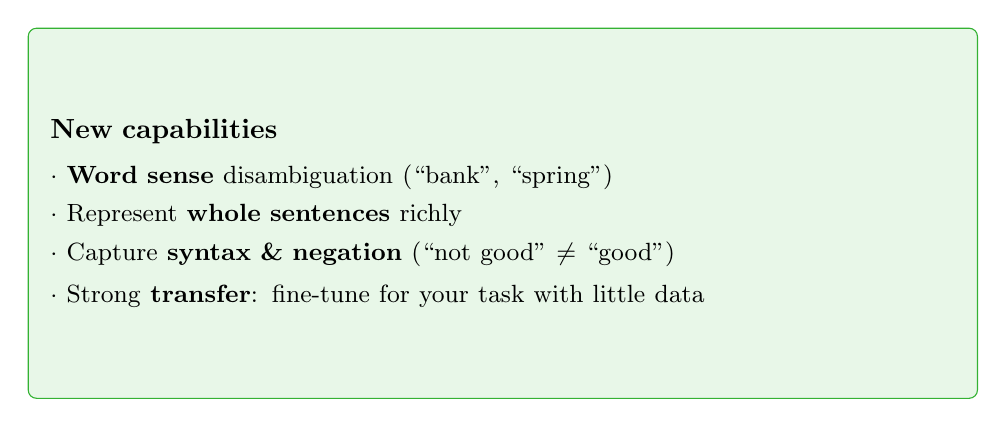
\begin{tikzpicture}
    \node[fill=lightgreen, draw=wurgreen, rounded corners=3pt,
          inner xsep=8pt, inner ysep=8pt, text width=\columnwidth-18pt, minimum height=4.7cm]{%
      \textbf{New capabilities}\\[5pt]
      {\small
      $\cdot$ \textbf{Word sense} disambiguation (``bank'', ``spring'')\\[3pt]
      $\cdot$ Represent \textbf{whole sentences} richly\\[3pt]
      $\cdot$ Capture \textbf{syntax \& negation} (``not good'' $\neq$ ``good'')\\[3pt]
      $\cdot$ Strong \textbf{transfer}: fine-tune for your task with little data}};
  \end{tikzpicture}

  \column{0.48\textwidth}
  \vspace{0pt}
  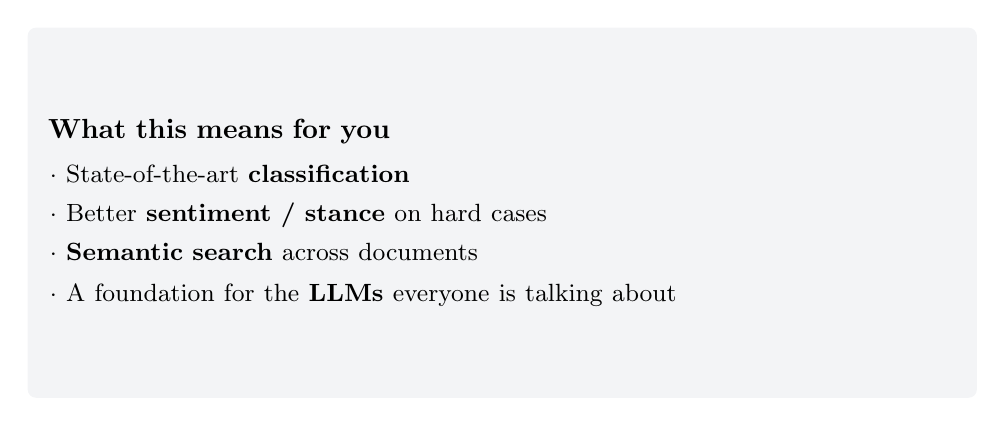
\begin{tikzpicture}
    \node[fill=lightgray, rounded corners=3pt,
          inner xsep=8pt, inner ysep=8pt, text width=\columnwidth-18pt, minimum height=4.7cm]{%
      \textbf{What this means for you}\\[5pt]
      {\small
      $\cdot$ State-of-the-art \textbf{classification}\\[3pt]
      $\cdot$ Better \textbf{sentiment / stance} on hard cases\\[3pt]
      $\cdot$ \textbf{Semantic search} across documents\\[3pt]
      $\cdot$ A foundation for the \textbf{LLMs} everyone is talking about}};
  \end{tikzpicture}
\end{columns}

\medskip
{\small\textcolor{midgray}{\textit{The jump from static to contextual is what took NLP from
``useful'' to ``everywhere'' over the last few years.}}}
\end{frame}

% ── SLIDE 4: the transformer arrives ──────────────────────────────────────
\begin{frame}{The Breakthrough: ``Attention Is All You Need''}
\vspace{0.2cm}
\begin{center}

\begin{tikzpicture}
  \node[fill=darknavy, rounded corners=3pt,
        inner xsep=12pt, inner ysep=10pt, text width=0.8\textwidth]{%
    {\centering\textcolor{white}{\large\textbf{``Attention Is All You Need''}}\\[3pt]
    \textcolor{midgray}{\small Vaswani et al., 2017 --- the paper that introduced the \textbf{transformer}}\par}};
\end{tikzpicture}
\end{center}

\bigskip
{\small Before 2017, models read text \textbf{word by word, in order} (recurrent networks) ---
slow, and forgetful over long distances. The transformer threw that out and replaced it with
one mechanism: \textbf{attention}, which lets every word look at every other word \textbf{at
once}.}

\medskip
{\small That single idea powers \textbf{BERT}, \textbf{GPT}, and essentially every modern
language model. The next few slides build up what ``attention'' actually means.}
\end{frame}

% ── SLIDE 5: attention intuition ──────────────────────────────────────────
\begin{frame}{Attention: The Core Intuition}
\vspace{0.2cm}
{\small To understand a word, you look at the \textbf{other words that give it meaning}.
Attention makes a model do exactly this --- for every word, it decides \textbf{how much to
focus on each other word} in the sentence.}

\medskip
\begin{center}
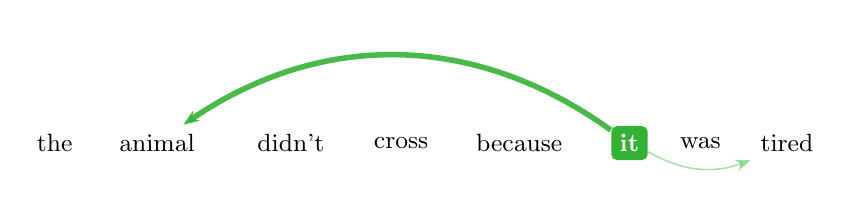
\begin{tikzpicture}[font=\small]
  \node (the) at (0,0) {the};
  \node (animal) at (1.3,0) {animal};
  \node (didnt) at (3.0,0) {didn't};
  \node (cross) at (4.4,0) {cross};
  \node (because) at (5.9,0) {because};
  \node (it) [fill=wurgreen, text=white, rounded corners=2pt, inner sep=3pt] at (7.3,0) {\textbf{it}};
  \node (was) at (8.2,0) {was};
  \node (tired) at (9.3,0) {tired};
  % attention arcs from "it"
  \draw[-{Stealth[length=2mm]}, wurgreen, line width=2pt, opacity=0.9] (it) to[bend right=35] (animal);
  \draw[-{Stealth[length=2mm]}, wurgreen, line width=0.6pt, opacity=0.4] (it) to[bend right=25] (tired);
\end{tikzpicture}
\end{center}

\medskip
{\small To represent \textbf{``it''}, the model pays \textbf{strong attention} to
\textbf{``animal''} (that is what ``it'' refers to) and a little to ``tired''. The thickness of
each arrow is the \textbf{attention weight} --- how relevant that word is.}

\medskip
{\small\textcolor{midgray}{\textit{Crucially, the model \emph{learns} these weights from data ---
nobody hand-codes that ``it'' means ``animal'' here.}}}
\end{frame}

% ── SLIDE 6: how attention works ─────────────────────────────────────────
\begin{frame}{How Attention Works --- Without the Math}
\vspace{0.15cm}
{\small For each word, attention runs a little \textbf{matching process}. A useful analogy is
\textbf{searching}:}

\medskip
\begin{columns}[T]
  \column{0.32\textwidth}
  \vspace{0pt}
  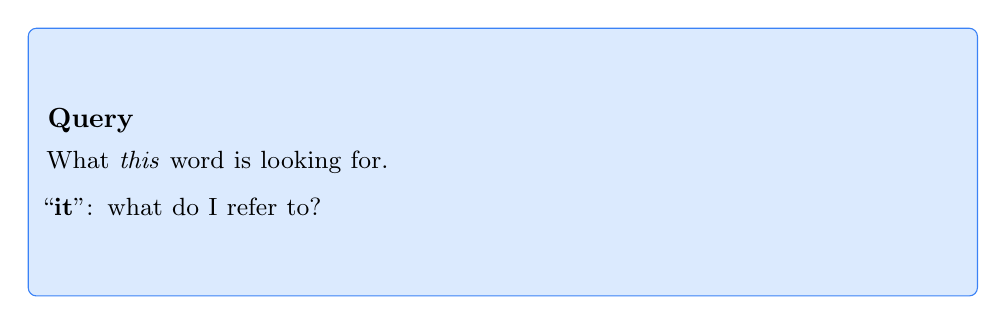
\begin{tikzpicture}
    \node[fill=attnblue, draw=attnborder, rounded corners=3pt,
          inner xsep=7pt, inner ysep=7pt, text width=\columnwidth-16pt, minimum height=3.4cm]{%
      \textbf{Query}\\[4pt]
      {\small What \emph{this} word is looking for.\\[5pt]
      ``\textbf{it}'': what do I refer to?}};
  \end{tikzpicture}

  \column{0.32\textwidth}
  \vspace{0pt}
  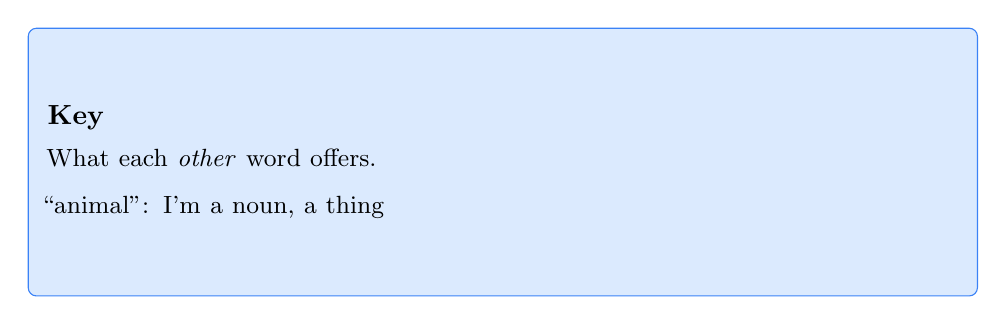
\begin{tikzpicture}
    \node[fill=attnblue, draw=attnborder, rounded corners=3pt,
          inner xsep=7pt, inner ysep=7pt, text width=\columnwidth-16pt, minimum height=3.4cm]{%
      \textbf{Key}\\[4pt]
      {\small What each \emph{other} word offers.\\[5pt]
      ``animal'': I'm a noun, a thing}};
  \end{tikzpicture}

  \column{0.32\textwidth}
  \vspace{0pt}
  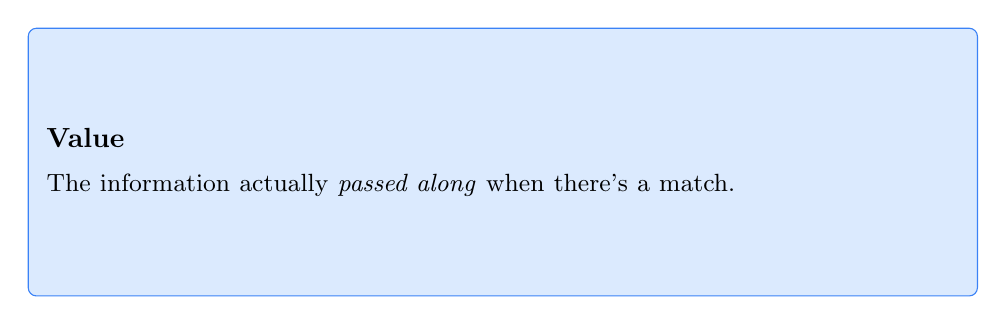
\begin{tikzpicture}
    \node[fill=attnblue, draw=attnborder, rounded corners=3pt,
          inner xsep=7pt, inner ysep=7pt, text width=\columnwidth-16pt, minimum height=3.4cm]{%
      \textbf{Value}\\[4pt]
      {\small The information actually \emph{passed along} when there's a match.}};
  \end{tikzpicture}
\end{columns}

\medskip
{\small The word's \textbf{query} is compared with every other word's \textbf{key}. Good
matches get high \textbf{attention weights}, and the matching words' \textbf{values} are blended
together to form the word's new, \textbf{context-aware} representation.}

\medskip
{\small\textcolor{midgray}{\textit{Query--key--value: the whole transformer is built by
stacking this one operation many times.}}}
\end{frame}

% ── SLIDE 7: self-attention + stacking ────────────────────────────────────
\begin{frame}{From One Layer to a Deep Model}
\vspace{0.2cm}
{\small Attention runs \textbf{in parallel} for every word (this is \textbf{self-attention} ---
the sentence attends to itself). Then we \textbf{stack many layers}, each refining the
representations further.}

\medskip
\begin{center}
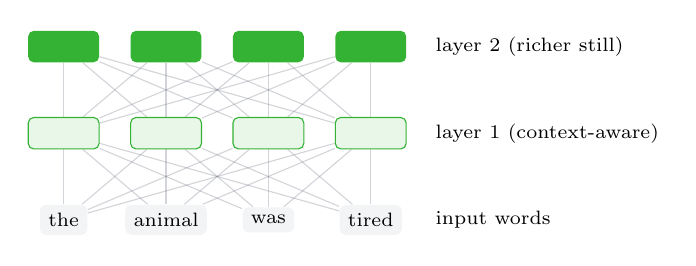
\begin{tikzpicture}[font=\scriptsize, node distance=0.35cm]
  % layer 0 (input words)
  \foreach \i/\w in {0/the, 1/animal, 2/was, 3/tired} {
    \node[fill=lightgray, rounded corners=2pt, inner sep=3pt] (l0-\i) at (1.3*\i,0) {\w};
  }
  % layer 1
  \foreach \i in {0,1,2,3} {
    \node[fill=lightgreen, draw=wurgreen, rounded corners=2pt, minimum width=0.9cm, minimum height=0.4cm] (l1-\i) at (1.3*\i,1.1) {};
  }
  % layer 2
  \foreach \i in {0,1,2,3} {
    \node[fill=wurgreen, rounded corners=2pt, minimum width=0.9cm, minimum height=0.4cm] (l2-\i) at (1.3*\i,2.2) {};
  }
  % connections (each to each)
  \foreach \a in {0,1,2,3} {
    \foreach \b in {0,1,2,3} {
      \draw[midgray, opacity=0.3] (l0-\a) -- (l1-\b);
      \draw[midgray, opacity=0.3] (l1-\a) -- (l2-\b);
    }
  }
  \node[right, font=\scriptsize] at (4.6,0) {input words};
  \node[right, font=\scriptsize] at (4.6,1.1) {layer 1 (context-aware)};
  \node[right, font=\scriptsize] at (4.6,2.2) {layer 2 (richer still)};
\end{tikzpicture}
\end{center}

\medskip
{\small Each layer lets every word gather information from all the others. After a dozen
layers, each word's vector reflects the \textbf{entire sentence}. \textbf{BERT} has 12 such
layers; large models have many more.}
\end{frame}

% ── SLIDE 8: BERT pretraining ─────────────────────────────────────────────
\begin{frame}{How BERT Learns: Masked Language Modeling}
\vspace{0.2cm}
{\small A transformer needs to be \textbf{trained} on something. \textbf{BERT}
--- \textit{Bidirectional Encoder Representations from Transformers} (Devlin et al., 2018) ---
uses a clever self-supervised task: \textbf{fill in the blank}.}

\medskip
\begin{center}
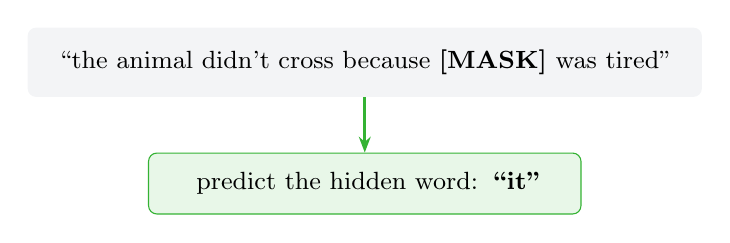
\begin{tikzpicture}[font=\small]
  \node[fill=lightgray, rounded corners=3pt, inner sep=8pt, text width=8cm, align=center] (masked)
    {``the animal didn't cross because \textbf{[MASK]} was tired''};
  \node[fill=lightgreen, draw=wurgreen, rounded corners=3pt, inner sep=7pt,
        text width=5cm, align=center, below=0.7cm of masked] (pred)
    {predict the hidden word: \textbf{``it''}};
  \draw[-{Stealth[length=2mm]}, wurgreen, line width=1pt] (masked) -- (pred);
\end{tikzpicture}
\end{center}

\medskip
{\small Hide ~15\% of words and train the model to \textbf{predict them from context}. To do
this well, it \emph{must} learn grammar, meaning, and world knowledge --- all \textbf{without
human labels}.}

\smallskip
{\small The \textbf{``Bidirectional''} in the name matters here: to guess the blank, BERT reads
the words \emph{both before and after} it --- unlike left-to-right models that only look back.
\textcolor{midgray}{\textit{(The same ``fake task'' trick as Word2Vec, but far more powerful.)}}}
\end{frame}

% ── SLIDE 9: encoders vs decoders ─────────────────────────────────────────
\begin{frame}{Two Families: Encoders and Decoders}
\vspace{0.3cm}
\begin{columns}[T]
  \column{0.48\textwidth}
  \vspace{0pt}
  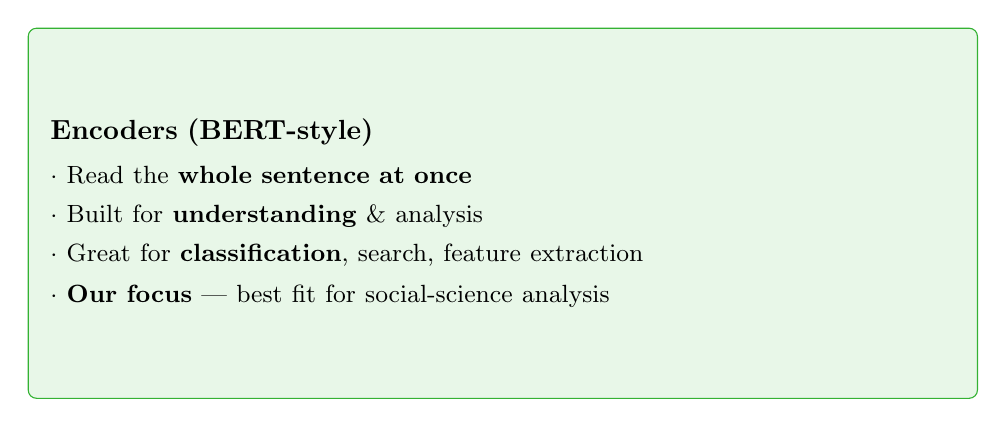
\begin{tikzpicture}
    \node[fill=lightgreen, draw=wurgreen, rounded corners=3pt,
          inner xsep=8pt, inner ysep=8pt, text width=\columnwidth-18pt, minimum height=4.7cm]{%
      \textbf{Encoders (BERT-style)}\\[5pt]
      {\small
      $\cdot$ Read the \textbf{whole sentence at once}\\[3pt]
      $\cdot$ Built for \textbf{understanding} \& analysis\\[3pt]
      $\cdot$ Great for \textbf{classification}, search, feature extraction\\[3pt]
      \textbf{$\cdot$ Our focus} --- best fit for social-science analysis}};
  \end{tikzpicture}

  \column{0.48\textwidth}
  \vspace{0pt}
  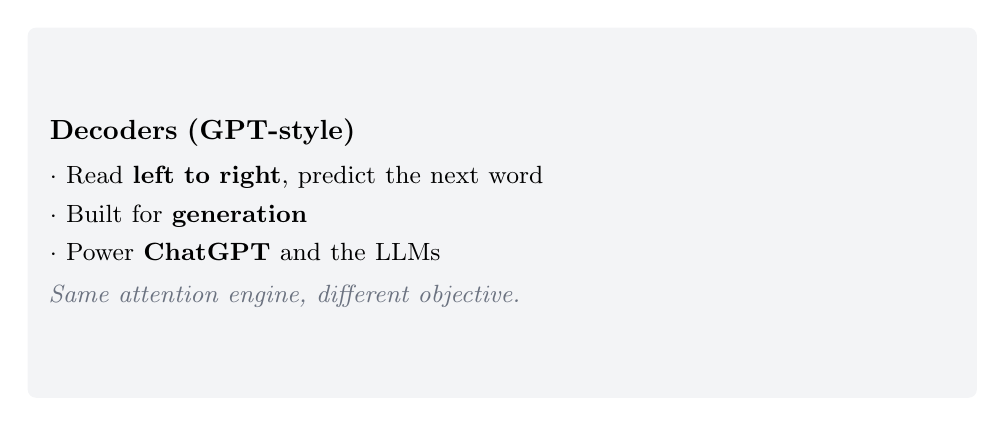
\begin{tikzpicture}
    \node[fill=lightgray, rounded corners=3pt,
          inner xsep=8pt, inner ysep=8pt, text width=\columnwidth-18pt, minimum height=4.7cm]{%
      \textbf{Decoders (GPT-style)}\\[5pt]
      {\small
      $\cdot$ Read \textbf{left to right}, predict the next word\\[3pt]
      $\cdot$ Built for \textbf{generation}\\[3pt]
      $\cdot$ Power \textbf{ChatGPT} and the LLMs\\[3pt]
      \textcolor{midgray}{\textit{Same attention engine, different objective.}}}};
  \end{tikzpicture}
\end{columns}

\medskip
{\small\textcolor{midgray}{\textit{For \emph{measuring} and \emph{classifying} text --- what
social scientists usually want --- encoders like BERT are typically the right tool.}}}
\end{frame}

% ── SLIDE 10: recap ───────────────────────────────────────────────────────
\begin{frame}{Mechanics: The Takeaways}
\vspace{0.25cm}
\begin{itemize}\setlength\itemsep{7pt}
  \item[\textcolor{wurgreen}{\faCheck}]
    \textbf{Contextual embeddings} give a word a \textbf{different vector in each sentence} ---
    solving the ``bank'' problem
  \item[\textcolor{wurgreen}{\faCheck}]
    They are built on the \textbf{transformer} (``Attention Is All You Need'', 2017)
  \item[\textcolor{wurgreen}{\faCheck}]
    \textbf{Attention} lets each word focus on the other words that matter ---
    via \textbf{query, key, value}
  \item[\textcolor{wurgreen}{\faCheck}]
    \textbf{BERT} learns by \textbf{masked language modeling}: fill in the blank, no labels needed
  \item[\textcolor{wurgreen}{\faCheck}]
    \textbf{Encoders} (BERT) are for understanding; \textbf{decoders} (GPT) are for generation
\end{itemize}

\medskip
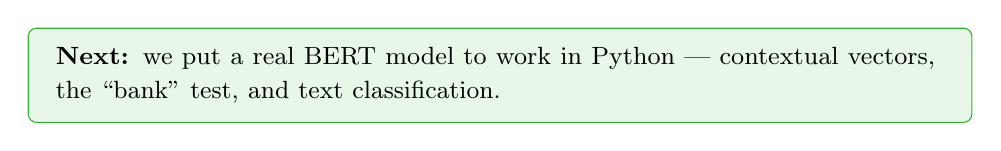
\begin{tikzpicture}
  \node[fill=lightgreen, draw=wurgreen, rounded corners=3pt,
        inner xsep=10pt, inner ysep=7pt, text width=\textwidth-24pt]{%
    {\small \textbf{Next:} we put a real BERT model to work in Python --- contextual vectors,
    the ``bank'' test, and text classification.}};
\end{tikzpicture}
\end{frame}

\end{document}
